
\section{SMA-Steckverbinder}
\label{section:steckverbinder_sma}
\begin{frame}%STARTCONTENT
Einsatz: Dort, wo man wenig Platz hat, auch bei hohen Frequenzen


\begin{figure}
    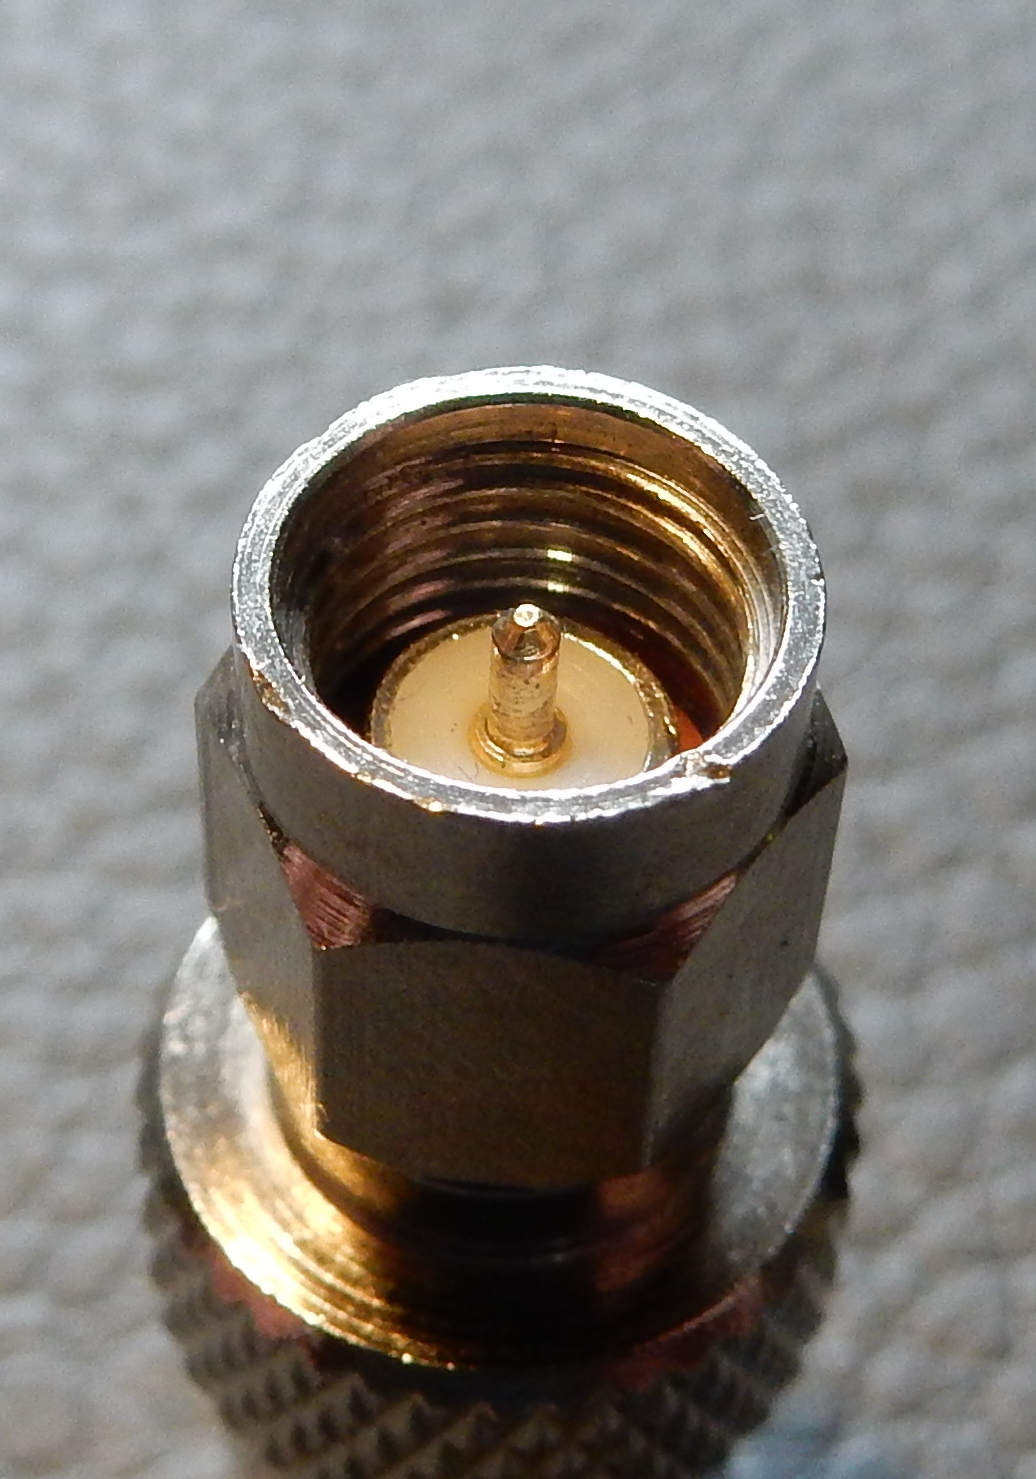
\includegraphics[width=0.85\textwidth]{foto/74}
    \caption{\scriptsize SMA-Stecker, hier stark vergrößert}
    \label{n_koaxsteckverbinder_sma}
\end{figure}

\end{frame}

\begin{frame}
\only<1>{
\begin{PQuestion}{NG205}{Welches HF-Steckverbindungs-System wird in der folgenden Darstellung gezeigt? }{PL}
{SMA}
{N}
{BNC}
{\DARCimage{1.0\linewidth}{611include}}\end{PQuestion}

}
\only<2>{
\begin{PQuestion}{NG205}{Welches HF-Steckverbindungs-System wird in der folgenden Darstellung gezeigt? }{PL}
{\textbf{\textcolor{DARCgreen}{SMA}}}
{N}
{BNC}
{\DARCimage{1.0\linewidth}{611include}}\end{PQuestion}

}
\end{frame}

\begin{frame}
\only<1>{
\begin{QQuestion}{NG206}{Welche der folgenden HF-Steckverbindungs-Systeme sind für hohe Frequenzen (oberhalb \qty{300}{\MHz}) am besten geeignet?}{BNC und Cinch}
{UHF und BNetzA}
{N und SMA}
{Cinch und SMA}
\end{QQuestion}

}
\only<2>{
\begin{QQuestion}{NG206}{Welche der folgenden HF-Steckverbindungs-Systeme sind für hohe Frequenzen (oberhalb \qty{300}{\MHz}) am besten geeignet?}{BNC und Cinch}
{UHF und BNetzA}
{\textbf{\textcolor{DARCgreen}{N und SMA}}}
{Cinch und SMA}
\end{QQuestion}

}
\end{frame}%ENDCONTENT
